\subsection{Implementation and integration}
In this part will be presented the steps in order to implement and integrate the DREAM project. Here is our plan route : 

We will first start by creating component by component trying to obtain as soon a possible a first viable solution that some users will be able to use to have feedback on the application. For instance it will be useless to develop all the application and see at the end that it will not be used by farmers because it is not ergonomic and too complicated.

For this two servers will be used : a testing server and deployment server. First people will build the application on the test server and when some viable functionality are present push it to the production server. This will be used for testing by some selected users (farmers and policy makers). To do that first of all a continuous integration will be effective with a continuous delivery. When push code on the development server all the test will be run before that the new code is accepted.

We will bring development and operation teams together using the devops practice. Devops require more work at the beginning but will permit a better work.

So here will be the beginning for putting into place the DevOps process flow.
\begin{enumerate}
	\item Use an agile development process
	\item Adapt the processes for continuous integration and continuous delivery
	\item Automate the software development
	\item Automate the software testing
	\item All this using continuous deployment
\end{enumerate}

\begin{figure}[H]
	\centering
	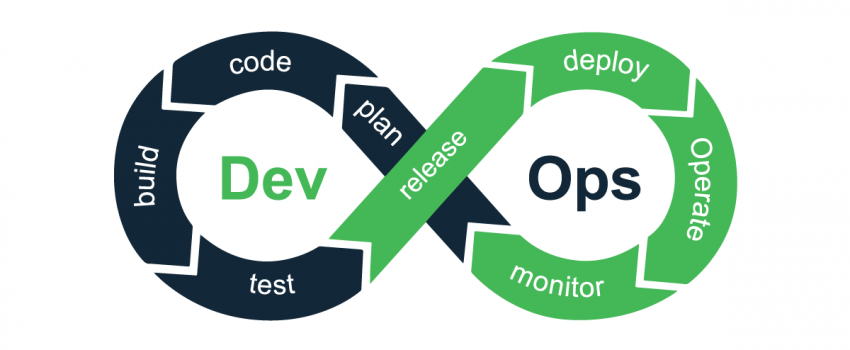
\includegraphics[width=0.8\columnwidth]{Images/schema-devops.png}
	\caption{DevOps schema}
	\label{Fig:devopsschema}
\end{figure}

After the setup of the DevOps process flow the application will be built trying to follow the following order. Of course as we use DevOps, changes can and will be made, so we can see the following as a guideline (see figure for the components \ref{fig:component_diag}).

\begin{enumerate}
	\item Make available some components to make a first version like Authentication, Release, Visualization, mails and the different databases related to them, data Encryption (important part but as it is not visible from the user point of view can be done after)
	\item forum
	\item messages
	\item calendar and localization
\end{enumerate}
All this using continuous deployment and taking into account the feedback from users, operators ...
Once a good system is present and that all the security and privacy is taken into account the development server will be shared to a bigger number of person. Until it is consider ready to be used by all, at that point it will used in all the state.
\subsection{Test Plan}
Testing should be done during all steps of implementations and integration.

Unit testing should be done for all the individual parts that will be developed. And if possible should be done by another person than whom did the code. Each part have to be tested individually to be sure that they can be used in other parts without errors and bugs. When a new component or change in done in a part all the previous Unit test should be run for the whole part. And in the case other parts are related also for the other parts.

At the same time global tests should be performed testing the good working of parts together. The tests will be run automatically before each deployment on the test and production server. To ensure proper implementation and integration of the DREAM system.